


\chapter{Observations}
  \label{ch_rbsp}

\todo{You know what would be great for putting this numerical work in context? A nice, consistent survey that breaks down the occurrence rate of Pc4 pulsations by harmonic, etc. }

\todo{There have been some surveys in the past. Dai did a nice one last year, but his filter biased him against the fundamental mode. And only a few past works have even worried about harmonic mode... probably because it's hard to get that information unless you have both E and B. }

\todo{Furthermore, it's awkward that Pgs are identified by visual inspection. How can we say how rare they are if they aren't rigorously defined? }

%Observations show that the poloidal mode is most excited in the second harmonic\cite{cummings_1969,hughes_1978,arthur_1981,singer_1982,takahashi_1984,engebretson_1988} even when there is a strong compressional component\cite{takahashi_1987,haerendel_1999,vaivads_2001,sibeck_2012}. 

% -----------------------------------------------------------------------------
% -----------------------------------------------------------------------------
% -----------------------------------------------------------------------------
\section{Event Selection}

\todo{Scroll through the entire almost-three-year duration of the Van Allen Probes mission so far. Both probes. }

\todo{Spinfit the field measurements to clean them up. This gives a ten-second cadence. Events are half an hour long to ensure that there are enough points to get a decent DFT. }

\todo{Also take $\vec{E} \cdot \vec{B} = 0$ to clean up the electric field. Notably, Dai did not do this (since he did not need the electric field). Any data within \SI{15}{\degree} of the probe's spin axis is discarded as part of this process. This is a significant portion of the data --- about half --- and furthermore introduces a bias in MLT, as discussed in \cref{sec_mlt}. Map the field to GSE coordinates to be consistent with the probe's position. }

\todo{Take a ten-minute rolling average of the data to get the background magnetic field. Subtract it out, and set $\zhat \parallel \vec{B_0}$. Then get the azimuthal direction with $\yhat \parallel \vec{B_0} \times \vec{r}$. The third component is the crosswise direction, $\xhat \equiv \yhat \times \zhat$. This is the same technique described by Liu\cite{liu_2010}. }

\todo{Compute discrete Fourier transforms: \dft{E_x}, \dft{E_y}, \dft{B_x^*}, \dft{B_y^*}. Then get the poloidal and toroidal Poynting flux, mapped to the ionosphere (giving a factor of $L^3$ for the compression of the flux tube). }
\begin{align}
  \dft{S_P} &\equiv -\frac{L^3}{\mz} \dft{E_y} \dft{B_x^*} &
  \dft{S_T} &\equiv \frac{L^3}{\mz} \dft{E_x} \dft{B_y^*}
\end{align}

\todo{Find the largest IMAGINARY component of the Poynting flux. This is the biggest standing wave present in this half hour. }

\todo{Threshold on frequency: anything not in the Pc4 frequency range gets tossed. }

\todo{Threshold on magnitude: anything below \SI{e-2}{\mW/\m\squared} gets tossed. }

\todo{Threshold on coherence: if \dft{E} and \dft{B^*} aren't coherent at 0.9 or better, the event gets tossed. . }

\todo{Notably, there is NO threshold on spectral width. Broadband and messy signals are allowed. See \cref{fig_fwhm}. }

\todo{We try not to worry too much about first vs third harmonic, since we can't tell them apart except by guessing at frequency. Chisham and Orr\cite{chisham_1991} argue that around \SI{7}{\RE}, frequency around \SI{10}{\mHz} precludes higher harmonics. Or maybe look at \cite{green_1985}? }

%Green\cite{green_1979} and Cummings\cite{cummings_1969} talk about the frequencies for ideal toroidal modes. 

% -----------------------------------------------------------------------------
% -----------------------------------------------------------------------------
% -----------------------------------------------------------------------------
\section{Bias in MLT}
  \label{sec_mlt}

\todo{RBSP precesses over time. It took about 22 months to go all the way around Earth. In principle, this gets rid of any bias in MLT. However, because the spin plane faces the sun, we lose more data to $\vec{E} \cdot \vec{B} = 0$ on the flanks. }

\todo{It's not worth trying to get uniform coverage, then. We instead go for all available data. Almost 3 years of data from each probe. }

\todo{This comes out to ... probe-days between $L=4$ and $L=6$. Comparable to about a year from a ground magnetometer? }

\todo{The plots in section ... are normalized by \cref{fig_pos}. This is as close as we can get to cutting out the bias. }

\begin{figure}[!htb]
    \centering
    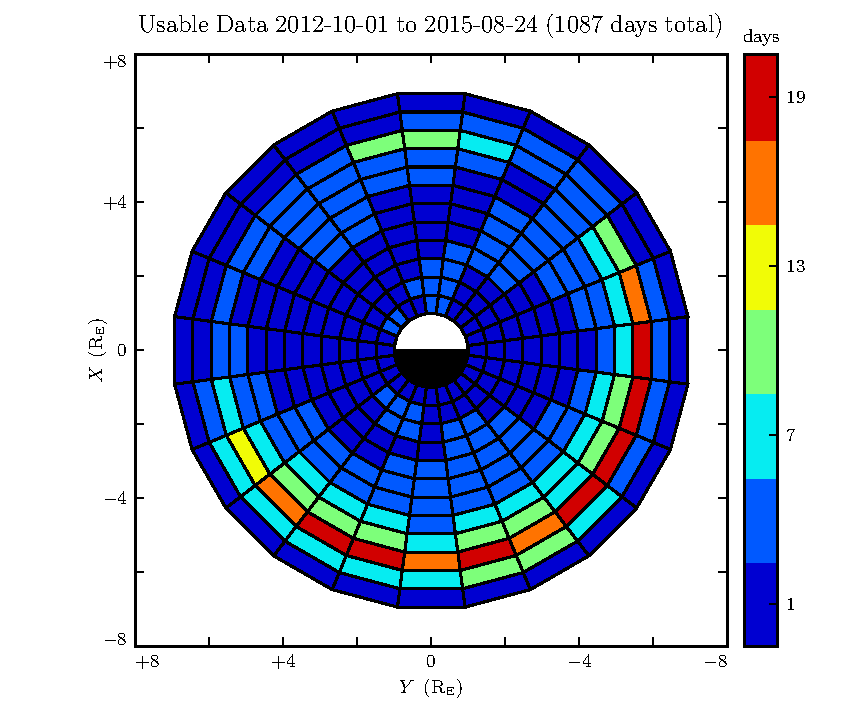
\includegraphics[width=\textwidth]{figures/pos.pdf}
    \caption[Spatial Distribution of Usable Van Allen Probe Data]{
      Electric field data is cleaned up by taking $\vec{E} \cdot \vec{B} = 0$. If the field is within \SI{15}{\degree} of the spin axis, that assumption is not reliable, so the data is discarded. Doing so biases the sample against the flanks. (The concentration near $L=6$ is due to the probes' slower movement near apogee.)
    }
    \label{fig_pos}
\end{figure}

% -----------------------------------------------------------------------------
% -----------------------------------------------------------------------------
% -----------------------------------------------------------------------------
\section{Slicing Events One Way...}

\begin{figure}[!htb]
    \centering
    
\includegraphics[width=\textwidth]{figures/placeholder.jpg}
    \caption[Distribution of Events by Spectral Width]{
      \todo{Break into three bins by FWHM. }
    }
    \label{fig_fwhm}
\end{figure}

% -----------------------------------------------------------------------------
% -----------------------------------------------------------------------------
% -----------------------------------------------------------------------------
\section{Slicing Events Another Way...}

\todo{Of the \about100 events where both the poloidal and toroidal channels triggered independently, almost all had one odd mode and one even mode. }

\todo{Collections of events at a single ground observatory (near \SI{66}{\degree}) over significant periods of time: }

Brekke\cite{brekke_1987} looked at 523 giant pulsation events recorded at Troms{\o}, Norway, from 1929 to 1985. This spanned several solar cycles. 

Rolf\cite{rolf_1931} collected 28 events between 1921 and 1930 at Abisko. 

Sucksdorf\cite{sucksdorff_1939} got 150 events between 1914 and 1938 in Sodankyl{\"a}. 

Harang\cite{harang_1941}. 97 events from 1929 to 1941. Also Troms{\o}. Note that this may have been limited by the war! 

This comes out to something like ... events over ... years. That's about ... giant pulsations per year, observed on the ground. 

\todo{Collections of events at an array of ground observatories: }

Chisham and Orr\cite{chisham_1991} found 34 events from 1984 to 1987 using the EISCAT magnetometer array in scandanavia. About \SI{5}{\degree} in MLT, decent coverage from \SIrange{63}{67}{\degree} mlat. This coincides with a solar minimum. 

Motoba, in 2015, recorded 105 giant pulsation events. The observations were carried out by a number of ground magnetometers spanning $\sim \SI{90}{\degree}$ in local time and ranging roughly \SIrange{60}{70}{\degree} magnetic latitude\cite{motoba_2015}. This was mostly during a period of low solar activity, so we expect a high count. 

\todo{Estimate of the size of an event's footprint:}

Velkamp\cite{veldkamp_1960} looked at a single large event and showed that, at best, it was visible over a span of \SI{5}{\degree} in magnetic latitude. 

This is seemingly consistent with the 29 February 2012 event discussed in detail by Motoba\cite{motoba_2015} --- Motoba shows some data, but doesn't discuss this aspect in detail. 

Takahashi\cite{takahashi_2011} computes a FWHM of about 1 in L, or \SI{2}{\degree} magnetic latitude. 

\todo{Tying that in to RBSP observations? }

Note that it's a bit tricky to compare ground observations to in situ observations. Large-\azm events won't make it through the ionosphere. 

There should be no bias with respect to MLT between a ground magnetometer and RBSP. Dai's analysis was specifically chosen to take advantage of the fact that RBSP's orbit had precessed all the way around the Earth. No preferred direction. And mlat shouldn't cause issues... these are FLRs, after all. 

How strong does an event need to be on the ground, or in the sky, to count as a giant pulsation? Motoba 2015\cite{motoba_2015} has an event which tops out on the order of \SI{10}{\nT} on the ground. It's more like \SI{5}{\mV/\m} in situ. Takahashi\cite{takahashi_2011} has similar values. 

Note that Takahashi\cite{takahashi_2013} has shown that it's OK to call something a giant pulsation even if it's not visible on the ground... though, obviously, we are comparing to ground magnetometer data for occurrence rate. 

If peak Pg observations are at $\SI{66}{\degree}$ mlat, that corresponds to $L = 6$. Then let's suppose that peak Pg viewing is $\SI{5}{\degree}$ wide --- estimating from the work of Velkamp and Motoba. That means RBSP should see lots of Pgs when it's between $L = 5.2$ andn $L = 7.1$. Well, \SI{7.1}{\RE} is outside its apogee, but the probes spend a fair amount of time outside $L = 5.2$, since they are moving pretty slowly at that point. 

Giant pulsations have been shown to be more numerous in times of low solar activity. That was the whole point of Brekke's seminal 1987 paper, and it's consistent with what we show in \cref{sec_pgs}. The RBSP observations occur during peak solar times, though it's an anemic solar peak\cite{pesnell_2016}. 

\todo{How much time does RBSP spend outside of $L = 5.2$ (for a range of \SI{5}{\degree})? How about $L = 5.6$ to $L = 6.5$ (for FWHM of \SI{2}{\degree}? }

Each RBSP probe spends about \SI{30}{\percent} of its orbit between $L = 5.6$ and $L = 6.5$. 

RBSP-A and RBSP-B count as two observers. In one $\sim 5$ cases out of hundreds do they simultaneously observe a poloidal Pc4 event (although, most notably for the 2012 event which \cite{dai_2013} considers in detail), both probes do fly through the same apparent event several hours apart from one another. 

The duration of Dai's survey is October 2012 to June 2014. Scaled by 2 probes, each of which is present in the peak Pg lshells 30\% of the time, that comes out to almost exactly one year. 

\todo{How many fundamental mode poloidal events do we see? How many could pass for giant pulsations? How many should we expect to see? }

\todo{How weird is it for a fundamental mode poloidal Pc4 to be monochromatic? }

\todo{How weird is it for a fundamental mode poloidal Pc4 to be stronger than \SI{5}{\mV/\m} at the equator? }






